\documentclass{elsarticle}
\usepackage{graphicx} % Required for inserting images
\usepackage{amsmath}
\usepackage{amssymb}
\usepackage{enumerate}
\usepackage{xcolor}

\begin{document}

\section*{Problemas}

\begin{enumerate}

%Ejercicio 1 RESUELTO
    \item[1.] (1 punto) Demuestra que la velocidad mas probable de una molecula de gas ideal es \(v_{p} = \sqrt{\frac{2K_{B}T}{m}}\), i.e., encuentra los extremos de la distribucion isotropica:
    \[
    P(v,v+dv) = 4\pi v^{2}f(v)
    \]

\color{purple}\textit{Answer.}\color{black} \[
\frac{d}{dv} [ 4\pi v^2 f(v) ] = 0.
\]

La función de distribución de velocidades de Maxwell-Boltzmann en una dimensión es:

\[
f(v) = \left( \frac{m}{2\pi k_B T} \right)^{3/2} e^{- \frac{m v^2}{2 k_B T}}.
\]

Sustituyéndola en la distribución isotrópica:

\[
P(v) = 4\pi v^2 \left( \frac{m}{2\pi k_B T} \right)^{3/2} e^{- \frac{m v^2}{2 k_B T}}.
\]

Derivamos esta función con respecto a \( v \):

\[
\frac{dP}{dv} = 4\pi \left( \frac{m}{2\pi k_B T} \right)^{3/2} \frac{d}{dv} \left[ v^2 e^{- \frac{m v^2}{2 k_B T}} \right].
\]

Usamos la regla del producto:

\[
\frac{d}{dv} \left[ v^2 e^{- \frac{m v^2}{2 k_B T}} \right] = 2v e^{- \frac{m v^2}{2 k_B T}} + v^2 e^{- \frac{m v^2}{2 k_B T}} \left(- \frac{m v}{k_B T} \right).
\]

Factorizamos \( e^{- \frac{m v^2}{2 k_B T}} \):

\[
\left( 2v - \frac{m v^3}{k_B T} \right) e^{- \frac{m v^2}{2 k_B T}} = 0.
\]

Para que esta ecuación se cumpla, el término entre paréntesis debe ser cero:

\[
2v - \frac{m v^3}{k_B T} = 0.
\]

Factorizamos \( v \):

\[
v \left( 2 - \frac{m v^2}{k_B T} \right) = 0.
\]

Descartamos la solución trivial \( v = 0 \) y resolvemos para \( v \):

\[
2 = \frac{m v^2}{k_B T}.
\]

Despejando \( v \):

\[
v_p = \sqrt{\frac{2 k_B T}{m}}.
\]

%Ejercicio 2 RESUELTO
    \item[2.] (1 punto) Muestra ahora que la velocidad promedio es \(\overline{v} = \int vf(v)d^{3}v = \sqrt{\frac{8k_{B}T}{\pi m}}\). Puedes utilizar la ecuacion (2) de las notas adjuntas. \\
    \color{purple}\textit{Answer.}\color{black} Dado que el ejercicio 3 me robó mi salud mental, ya no voy a pasar este a latex
\begin{figure}[h]
    \centering
    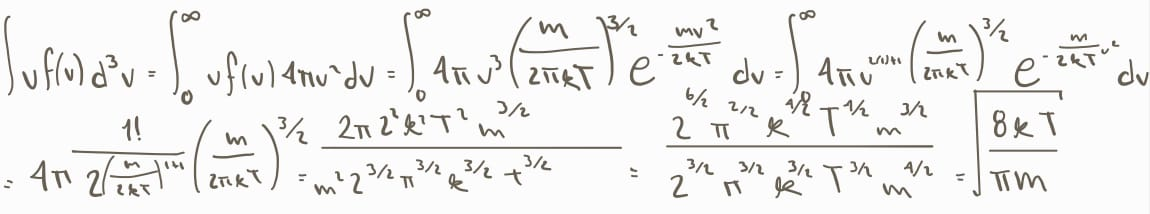
\includegraphics[width=1\linewidth]{procedimiento.jpg}
    \label{fig:enter-label}
\end{figure}

%Ejercicio 3 RESUELTO
    \item[3.] (2 pts) Un contenedor cubico contiene un mol de gas de argon a una temperatura de 293K.
    \begin{enumerate}
        \item ¿Cuantas moleculas tienen una velocidad entre 500 m/s y 510 m/s?
        \item ¿Cuantas moleculas tienen una velocidad entre 500 m/s y 510 m/s en una direccion particular? (integra ahora en coordenadas cartesianas utilizando el diferencial \(d^{3}v = dv_{x}dv_{y}dv_{z}\) y definiendo los limites de integracion adecuados para cada variable).
    \end{enumerate}

\color{purple}\textit{Answer.}\color{black} La distribución de velocidades moleculares está dada por la distribución de Maxwell-Boltzmann, que en tres dimensiones se expresa como:

\[
f(v) = \left(\frac{m}{2\pi k_B T} \right)^{3/2} 4\pi v^2 e^{-\frac{mv^2}{2k_B T}}
\]

El número de moléculas con velocidad entre \( v \) y \( v + dv \) está dado por:

\[
dN = N f(v) dv
\]

donde \( N = N_A \) (el número de moléculas en un mol de gas, es decir, el número de Avogadro).

a) Para encontrar el número de moléculas en este intervalo de velocidades, integramos la función de distribución en el rango \( 500 \leq v \leq 510 \):

\[
N_{500-510} = N_A \int_{500}^{510} f(v) dv
\]

Calculamos el coeficiente:

\[
\frac{m}{2k_B T} = \frac{6.63 \times 10^{-26}}{2 (1.38 \times 10^{-23} \times 293)} = \frac{6.63 \times 10^{-26}}{8.08 \times 10^{-21}} = 8.21 \times 10^{-6}
\]

Por lo que:

\[
\left( \frac{m}{2\pi k_B T} \right)^{3/2} = (8.21 \times 10^{-6})^{3/2} = 7.44 \times 10^{-9}
\]

Ahora, el exponente en la exponencial es:

\[
\frac{m v^2}{2 k_B T} = (8.21 \times 10^{-6}) v^2
\]

Para \( v = 500 \) m/s y \( v = 510 \) m/s:

\[
\frac{m v^2}{2 k_B T} \Big|_{v=500} = 8.21 \times 10^{-6} \times 500^2 = 2.05
\]

\[
\frac{m v^2}{2 k_B T} \Big|_{v=510} = 8.21 \times 10^{-6} \times 510^2 = 2.14
\]

Por lo tanto:

\[
f(500) = 7.44 \times 10^{-9} \times 4\pi (500)^2 e^{-2.05} = 2.99 \times 10^{-3}
\]

\[
f(510) = 7.44 \times 10^{-9} \times 4\pi (510)^2 e^{-2.14} = 2.83 \times 10^{-3}
\]

Aproximando la integral como \( f(505) \times \Delta v \):

\[
N_{500-510} \approx N_A \times (2.91 \times 10^{-3}) \times 10 = (6.022 \times 10^{23}) \times (2.91 \times 10^{-3}) \times 10 = 1.75 \times 10^{22}
\]

b) Ahora consideramos la distribución en coordenadas cartesianas. La distribución de Maxwell-Boltzmann en términos de las componentes de la velocidad es:

\[
f(v_x, v_y, v_z) = \left( \frac{m}{2\pi k_B T} \right)^{3/2} e^{-\frac{m(v_x^2 + v_y^2 + v_z^2)}{2 k_B T}}
\]

El número de moléculas con velocidades en el intervalo \( 500 \leq v \leq 510 \) en una dirección específica requiere transformar la distribución a coordenadas cartesianas y considerar el volumen diferencial \( d^3v = dv_x dv_y dv_z \).  

Para velocidades en una dirección particular (por ejemplo, solo en \( v_x \)), integramos sobre \( v_y \) y \( v_z \). Para pequeños intervalos de \( v \), la contribución angular es proporcional a:

\[
\frac{\Delta v}{v}
\]

Por lo que el número de moléculas en el intervalo en una única dirección se obtiene dividiendo el resultado del inciso (a) por $4\pi$:

\[
N_{\text{dirección}} \approx \frac{N_{500-510}}{4\pi} = \frac{1.75 \times 10^{22}}{12.56} = 1.39 \times 10^{21}
\]

%Ejercicio 4 a) RESUELTO c)
    \item[4.] (3 ptos) La densidad de energia de radiacion (por unidad de volumen, por unida de area) de Planck parametrizada utilizando la longitud de onda \(\lambda\), puede escribirse como:
    \[
    u(\lambda,T) = \frac{2hc}{\lambda^{5}} \frac{1}{e^{hc/(\lambda k_{B}T)} - 1} d\lambda
    \]
    \begin{enumerate}
        \item Muestre que la densidad espectral de la radiacion de cuerpo negro tiene un maximo para cada temperatura, que ocurre a la longitud de onda:
        \[
        \lambda_{m} = \frac{2\pi c \bar{}h}{4.965k_{B}T}
        \]
        \item Calcule ahora la maxima frecuencia \(\nu_{m}\) y muestre que \(\nu_{m}\neq c/\lambda_{m}\). Para ello utilice ahora la parametrizacion de frecuencia (\(\nu = c/\lambda\)):
        \[
        u(\nu,T) = u(\lambda,T) \frac{d\lambda}{d\nu} = \frac{2h\nu^{3}}{c^{2}} \frac{1}{e^{h\nu/k_{B}T} - 1} d\nu
        \]
        \item Si el sol presenta un maximo a \(\lambda_{m} \approx 5 \times 10^{3}\)A, ¿Cual es la temperatura de la superficie solar?
    \end{enumerate}

\color{purple}\textit{Answer.}\color{black} Dado que el máximo de emisión del Sol ocurre a \( \lambda_m \approx 5000 \) Å (o \( 5 \times 10^{-7} \) m), usamos la Ley de Wien del inciso a) pero sin el molesto h barra:

\[
\lambda_m T = \frac{hc}{4.965 k_B}.
\]

Sustituyendo valores numéricos:

\[
T = \frac{(6.626 \times 10^{-34} \text{ J·s}) (3.00 \times 10^8 \text{ m/s})}{(4.965) (1.381 \times 10^{-23} \text{ J/K}) (5.00 \times 10^{-7} \text{ m})} = \frac{1.988 \times 10^{-25}}{3.429 \times 10^{-29}} = 5787 \text{ K}.
\]

    %Ejercicio 5 RESUELTO
    \item[5.] (3 ptos) La ley de Stefan-Boltzmann nos dice que la energia radiada por un radiador de cuerpo negro por segundo, por unidad de superficie, es proporcional a la cuarta potencia de la temperatura absoluta y esta dada por:
    \[
    \frac{P}{A} = \sigma T^{4}
    \]
    con \(\sigma = 5,670 \times 10^{-8}\) W/m\(^{2}\)K\(^{4}\) la constante de Stefan. Tomando al Sol como un cuerpo negro a 5700 K, de radio \(R = 6,9634 \times 10^{8}\) m y masa total \(M \approx 1,989 \times 10^{30}\) kg:
    \begin{enumerate}
        \item ¿Cuanta potencia es radiada por un metro cuadrado de la superficie del sol?
        \item Determine la fraccion de su masa que emite anualmente como radiacion electromagnetica.
        \item Dado que la distancia a la Tierra es de aproximadamente 200 radios solares, ¿cual es la potencia maxima posible de una instalacion de energia solar de un kilometro cuadrado?
    \end{enumerate}
\end{enumerate}

\color{purple}\textit{Answer.}\color{black} a) La potencia emitida por metro cuadrado de la superficie del Sol se obtiene directamente sustituyendo a partir de la ecuación de Stefan-Boltzmann:

\[
P_{\text{m²}} = \sigma T^4  = (5.670 \times 10^{-8} \text{ W/m}^2\text{K}^4) (5700 \text{ K})^4
\]

Calculamos la potencia:

\[
P_{\text{m²}} = (5.670 \times 10^{-8}) \times (1.0569 \times 10^{15}) = 5.99 \times 10^7 \text{ W/m²}
\]

b) La potencia total radiada por el Sol se obtiene multiplicando la potencia por unidad de área por la superficie total del Sol. Como el Sol es aproximadamente esférico, su área superficial es:

\[
A_{\odot} = 4\pi R^2 = 4\pi (6.9634 \times 10^8)^2 = 4\pi (4.847 \times 10^{17}) = 6.09 \times 10^{18} \text{ m}^2
\]

La potencia total radiada es:

\[
P_{\odot} = P_{\text{m²}} \cdot A_{\odot} = (5.99 \times 10^7) \times (6.09 \times 10^{18}) = 3.65 \times 10^{26} \text{ W}
\]

Ahora, para determinar la fracción de la masa del Sol que se convierte en radiación electromagnética anualmente, calculamos la energía total emitida en un año. Como la potencia es la energía emitida por unidad de tiempo, usamos:

\[
E_{\odot} = P_{\odot} \times (\text{segundos en un año})
\]

El número de segundos en un año es simplemente:

\[
t_{\text{año}} = 365.25 \times 24 \times 3600 = 3.156 \times 10^7 \text{ s}
\]

Entonces:

\[
E_{\odot} = (3.65 \times 10^{26}) \times (3.156 \times 10^7) = 1.15 \times 10^{34} \text{ J}
\]

La equivalencia entre masa y energía está dada por la ecuación de la energía según la relatividad:

\[
E^2 = (pc)^2+(mc^2)^2
\]

Despejando la masa:

\[
m_{\text{emitida}} = \frac{E_{\odot}}{c^2} = \frac{1.15 \times 10^{34}}{(3.00 \times 10^8)^2} = \frac{1.15 \times 10^{34}}{9.00 \times 10^{16}} = 1.28 \times 10^{17} \text{ kg}
\]

La fracción de la masa del Sol que se convierte en energía anualmente es:

\[
\frac{m_{\text{emitida}}}{M_{\odot}} = \frac{1.28 \times 10^{17}}{1.989 \times 10^{30}} = 6.44 \times 10^{-14}
\]

c) Dado que la Tierra está a una distancia de aproximadamente 200 radios solares del Sol, la potencia que recibe la Tierra se puede determinar considerando que la energía se distribuye en una esfera de radio \( d = 200 R \).  

La superficie de esta esfera es:

\[
A_{\text{esfera}} = 4\pi d^2 = 4\pi (200 R)^2 = 4\pi (4 \times 10^4 R^2) = 1.57 \times 10^{10} A_{\odot}
\]

La potencia por unidad de área a esta distancia es:

\[
I_{\text{Tierra}} = \frac{P_{\odot}}{A_{\text{esfera}}} = \frac{3.65 \times 10^{26}}{1.57 \times 10^{10} \times 6.09 \times 10^{18}} = \frac{3.65 \times 10^{26}}{9.57 \times 10^{28}} = 3.81 \times 10^3 \text{ W/m}^2
\]

Si la instalación de energía solar tiene un área de \( 1km^2 \) (es decir, \( 10^6 m^2\)), la potencia máxima que podría recibir sería:

\[
P_{\text{instalación}} = I_{\text{Tierra}} \times 10^6 = (3.81 \times 10^3) \times 10^6 = 3.81 \times 10^9 \text{ W} = 3.81 \text{ GW}
\]

\end{document}
